\documentclass[12pt]{article}

\usepackage[dvips,letterpaper,margin=0.75in,bottom=0.75in]{geometry}
\usepackage{cite}
\usepackage{slashed}
\usepackage{graphicx}
\usepackage{mathtools}
\usepackage{tikz}
\usepackage{arydshln}
\usepackage[compat=1.1.0]{tikz-feynman}
\usepackage{amsmath, amssymb, amsthm}
\usepackage{slashed}
\usepackage{bm}
\usepackage{braket}
\usepackage{hyperref}

\newcommand{\Tr}{\mathrm{Tr}}
\newcommand{\dd}{\mathrm{d}}

\begin{document}

\title{PHY 130B \\ Lecture Notes Q: \\
Quantum Chromodynamics\\}
\author{Michael Mulhearn}

\maketitle

\newcounter{exercise}
\setcounter{exercise}{0}

\newcommand{\exercise}{
\stepcounter{exercise}
\noindent
{\bf Exercise E.\theexercise:}
}

\section{The Need for Color}

In the homework we found that the  baryon is an
isospin quartet ($I=3/2$) with $J=3/2$ $\Delta^{++}$
composed of three up quarks,
\begin{equation*}
    \Delta^{++} = uuu, \qquad J^P = \tfrac{3}{2}^{+}, \qquad L = 0.
\end{equation*}
With $L=0$ the spatial wavefunction is symmetric, and by considering
$J_z=\pm 3/2$, the spin wavefunction
(e.g.\ $\ket{\uparrow\uparrow\uparrow}$) is also symmetric. The
overall wavefunction of three identical fermions appears therefore
appears to be symmetric under exchange --- in violation of
Fermi--Dirac statistics.  This suggest that quarks must carry an
additional quantum number, \emph{color}.  Each quark has three color
states,
\begin{equation*}
    q \;\longrightarrow\; q_R,\; q_G,\; q_B,
\end{equation*}
As we shall the see, the quarks are arranged in an antisymmetric color
singlet, so the total wave function is antisymmetric, conistent with
Fermi-Dirac statistics.

Further experimental evidence comes from $e^+e^-$ annihilation, with:
\begin{equation*}
    \sigma(e^+e^- \to f\bar f) \;=\; \frac{4\pi\alpha^2 Q_f^2}{3s},
\end{equation*}
where $Q_f$ is the electric charge of fermion $f$ in units of $e$, and
we have neglected final-state masses ($s \gg m_f^2$). The ratio of
cross-section for hadron production to muon production is:
\begin{equation*}
    R \;\equiv\; \frac{\sigma(e^+e^- \to \text{hadrons})}{\sigma(e^+e^- \to \mu^+\mu^-)}
       \;=\; \frac{\sum_f \sigma(e^+e^- \to q_f \bar q_f)}{\sigma(e^+e^- \to \mu^+\mu^-)}
       \;=\; 3 \sum_f Q_f^2,
\end{equation*}
where the sum runs over quark flavors kinematically accessible at
$\sqrt{s}$.  This shows that each quark flavor contributes a factor of
three to the cross-section, consistent with three quark flavors (each
contributing equally to the rate).

\section{SU(3) Gauge Symmetry}

Each quark flavor now carries a color index $i = 1,2,3$, and we collect the
three color states into a triplet:
\begin{equation*}
    \psi = \begin{pmatrix} \psi_1 \\ \psi_2 \\ \psi_3 \end{pmatrix},
    \qquad
    c_1 = R = \begin{pmatrix} 1 \\ 0 \\ 0 \end{pmatrix}, \quad
    c_2 = G = \begin{pmatrix} 0 \\ 1 \\ 0 \end{pmatrix}, \quad
    c_3 = B = \begin{pmatrix} 0 \\ 0 \\ 1 \end{pmatrix}.
\end{equation*}
We postulate invariance under global SU(3) rotations in color space,
\begin{equation*}
    \psi \;\longrightarrow\; \psi' = U\,\psi, \qquad U \in \mathrm{SU}(3),
\end{equation*}
with
\begin{equation*}
    U = \exp\!\big( i g_s\, \alpha^a\, T^a \big), \qquad T^a = \tfrac{1}{2}\lambda^a,
    \qquad a = 1,\ldots,8,
\end{equation*}
where $\lambda^a$ are the eight Gell-Mann matrices and $T^a$ are the
generators of SU(3) in the fundamental representation.  We already
encountered the Gell-Mann matrices when considering $u,d,s$ quark
flavor symmetry.\\[5pt]

\noindent
{\bf QED review:}
Let's first recall how QED emergies from local $U(1)$ symmetry.  We
promote a global symmetry to a local one, $\lambda \to
\lambda(x)$. The naive derivative no longer transforms covariantly:
\begin{equation*}
    \partial_\mu \psi \;\longrightarrow\; \partial_\mu (U\psi)
       = U \partial_\mu \psi + (\partial_\mu U)\,\psi,
\end{equation*}
so we introduce a covariant derivative $D_\mu$ that does:
\begin{equation*}
    D_\mu \psi \;\longrightarrow\; D'_\mu \psi' = U\, D_\mu \psi.
\end{equation*}
For U(1), $U = \exp(iQ e\, \lambda(x))$, and
\begin{equation*}
  D_\mu = \partial_\mu + i Q e\, A_\mu(x).
\end{equation*}
Requiring $D'_\mu \psi' = U D_\mu \psi$,
\begin{align*}
    \big(\partial_\mu + i Q e\, A'_\mu\big) U \psi
       &= U \big(\partial_\mu + i Q e\, A_\mu\big)\psi \\
    (\partial_\mu U)\psi + U \partial_\mu \psi + i Q e\, A'_\mu\, U \psi
       &= U \partial_\mu \psi + i Q e\, U A_\mu \psi.
\end{align*}
The $U \partial_\mu \psi$ terms cancel. Using $U^\dagger U = 1$ and noting $U$ is
a number (so it commutes with $A_\mu$),
\begin{equation*}
    i Q e\, A'_\mu \;=\; i Q e\, A_\mu - (\partial_\mu U)\, U^\dagger.
\end{equation*}
With $U = \exp(iQ e\, \lambda)$, $(\partial_\mu U)\, U^\dagger = i Q e\, \partial_\mu \lambda$, so
\begin{equation*}
    A_\mu \;\longrightarrow\; A'_\mu = A_\mu - \partial_\mu \lambda.
\end{equation*}
For a free particle, partial derivatives commute,
$[\partial_\mu, \partial_\nu] = 0$. With the gauge field,
\begin{equation*}
    [D_\mu, D_\nu]\, \psi
       = i Q e\,\big(\partial_\mu A_\nu - \partial_\nu A_\mu\big)\psi
         + (i Q e)^2\, [A_\mu, A_\nu]\,\psi,
\end{equation*}
and the $[A_\mu, A_\nu]$ piece vanishes because $A_\mu$ is a number. Thus
\begin{equation*}
    [D_\mu, D_\nu] = i Q e\, F_{\mu\nu},
\end{equation*}
with
\begin{equation}
    \qquad
    F_{\mu\nu} = \partial_\mu A_\nu - \partial_\nu A_\mu,
\end{equation}
and the source-free Maxwell equations follow from
\begin{equation}
  \partial_\mu F^{\mu\nu} = 0.
\end{equation}

\noindent
{\bf QCD:}
Following the same approach as our derivation of QED, we promote SU(3) to a local symmetry:
$$\alpha^a \to \alpha^a(x)$$
and so:
$$U = \exp(i g_s \alpha^a(x) T^a)$$
Under this transformation,
\begin{equation*}
    \psi \;\longrightarrow\; \psi' = U\,\psi,
\end{equation*}
and the derivative again picks up an extra term,
\begin{equation*}
    \partial_\mu \psi \;\longrightarrow\; \partial_\mu(U\psi)
       \;=\; U \partial_\mu \psi + (\partial_\mu U)\,\psi
       \;=\; U\big(\partial_\mu + i g_s (\partial_\mu \alpha^a)\, T^a\big)\psi,
\end{equation*}
The transformation of the derivative is therefore
\begin{equation*}
    \partial_\mu \;\longrightarrow\; \partial_\mu + i g_s (\partial_\mu \alpha^a)\, T^a.
\end{equation*}
We define a covariant derivative with a new gluon field $G^a_\mu(x)$ with a gauge freedom that cancels the additional term in the derivative:
\begin{equation}
 \label{eqn:covd-qcd}
    D_\mu \;=\; \partial_\mu + i g_s\, G^a_\mu(x)\, T^a.
\end{equation}
Requiring $D'_\mu \psi' = U D_\mu \psi$ with $\psi' = U\psi$ gives
\begin{align}
    \big( \partial_\mu + i g_s\, (G^a_\mu)' T^a \big) U\psi
       &= U \big( \partial_\mu + i g_s\, G^a_\mu T^a \big) \psi \\
    (\partial_\mu U)\psi + U \partial_\mu \psi + i g_s\, (G^a_\mu)' T^a\, U\psi
       &= U \partial_\mu \psi + i g_s\, U G^a_\mu T^a \psi.
\end{align}
Solving for $(G^a_\mu) T^a$:
\begin{equation}
  \label{eqn:gluon-transformation}
  G^a_\mu T^a \to (G^a_\mu)' T^a = G^a_\mu U T^a\, U^\dagger
  + \frac{i}{g_s}\,(\partial_\mu U)\, U^\dagger
\end{equation}
The first term is precisely the transformation that makes the generator $T^a$ 
term covariant:
\begin{equation}
T^a \psi \to \left( U T^a U^\dagger \right) \left(U \psi \right) = U T^a \psi
\end{equation}
and the second cancels the addition term from the transformation of the derivative.  This is much like for QED, except that there are eight gluon fields $G^a_\mu$.
Repeating the field-strength calculation with
$D_\mu = \partial_\mu + i g_s G^a_\mu T^a$,
\begin{equation*}
    [D_\mu, D_\nu] = i g_s\,\big(\partial_\mu G^a_\nu - \partial_\nu G^a_\mu\big) T^a
       + (i g_s)^2\, G^a_\mu G^b_\nu\, [T^a, T^b].
\end{equation*}
Now the commutator $[T^a, T^b]$ does \emph{not} vanish.  Defining
\begin{equation*}
    [D_\mu, D_\nu] \;\equiv\; i g_s\, G_{\mu\nu},
\end{equation*}
with
\begin{equation}
 \label{eqn:field-qcd}
G_{\mu\nu} \;=\; \big(\partial_\mu G^a_\nu - \partial_\nu G^a_\mu\big) T^a
                          \;+\; i g_s\, G^a_\mu G^b_\nu\, [T^a, T^b]
\end{equation}
The first piece is the photon-like part, present for each of the eight
gluons.  The second piece is new: with $[T^a, T^b] \neq 0$, the gluon
field strength contains a term quadratic in the gluon fields, which,
as we shall see, leads to gluon self-interactions.

\section{Quark--Gluon Interaction}

Promoting $\partial_\mu \to D_\mu$ in the free Dirac equation gives
\begin{equation*}
    i\gamma^\mu D_\mu \psi = m\psi
    \quad\Longrightarrow\quad
    i\gamma^\mu\!\left(\partial_\mu + i g_s\, G^a_\mu T^a\right)\psi = m\psi.
\end{equation*}
As before, we determine the interaction Hamiltonian from:
$$
i\,\frac{\partial \psi}{\partial t}
= \left( H^{(0)} + H_{\rm QCD} \right) \psi
$$
Isolating the time derivative from the Dirac equation:
\begin{equation*}
    i\,\frac{\partial \psi}{\partial t}
       = \left( m\gamma^0 - i\gamma^0\vec\gamma\cdot\vec\nabla
                + g_s\,\gamma^0 \gamma^\mu G^a_\mu T^a \right)\psi,
\end{equation*}
from which we read off
\begin{equation*}
    H_\text{QCD} \;=\; g_s\, \gamma^0 \gamma^\mu\, G^a_\mu(x)\, T^a.
\end{equation*}
where $g_s$ is the strength of the strong interaction (the color
charge), $G^a_\mu(x)$ is a real field (one for each of the eight
gluons), $T^a$ is a 3x3 matrix representing a linear operator in color
space, and the gamma matrices are 4x4 matrices that act on bispinors.
Nonetheless, the interaction term is quite similar to QED in
structcure, with the replacement
\begin{equation*}
    e\,Q\, A_\mu(x) \;\longrightarrow\; g_s\, G^a_\mu(x)\, T^a,
\end{equation*}

The plane-wave solutions are extended to include a definite color:
\begin{equation*}
    \psi_{p, i}(x) \;=\; u(p)\, c_i\, e^{-i p \cdot x},
    \qquad
    c_1 = r = \begin{pmatrix} 1 \\ 0 \\ 0 \end{pmatrix},\quad
    c_2 = g = \begin{pmatrix} 0 \\ 1 \\ 0 \end{pmatrix},\quad
    c_3 = b = \begin{pmatrix} 0 \\ 0 \\ 1 \end{pmatrix}.
\end{equation*}
The Dirac spinors satisfy the usual completeness relation
\begin{equation*}
    \sum_\text{spins} u(p)\, \bar u(p) \;=\; \slashed{p} + m,
\end{equation*}
and the color basis is complete as well:
\begin{equation*}
    \sum_{i=1}^{3} c_i\, c_i^\dagger \;=\; I
\end{equation*}
The plane waves for the gluon field are similar to the photon plane waves, except that there are eight of them:
\begin{equation*}
    G^a_\mu(x) \;=\; \sum_a \varepsilon^a_\mu(q)\, e^{-i q \cdot x},
\end{equation*}
with polarization vector $\varepsilon^a_\mu$ and adjoint color label
$a$. As in QED, the exponential factors at each vertex enforce
four-momentum conservation via a delta function when integrating over
space-time, but we won't repeat that calculation here.

For the fundamental vertex
\begin{center}
\begin{tikzpicture}
  \begin{feynman}
    \vertex (a) at (0,0) {$a$};
    \vertex [right=3cm of a](x);
    \vertex [above right=2cm and 3cm of x](b){$b$};
    \vertex [below right=2cm and 3cm of x](g){$q$};
    \vertex (a) at (0,0) {$a$};   
    \diagram*{
      (a) -- [fermion, edge label={$q, c_i$}] (x) -- [fermion,  edge label={$q, c_j$}] (b),
      (x) -- [gluon, edge label={$g$}] (g) 
    };
\end{feynman}
\end{tikzpicture}
\end{center}
we have therefore:
\begin{align*}
    \big\langle b, j \,\big|\, H_\text{QCD} \,\big|\, a, i \big\rangle
       &= \bar u(b)\, c_j^\dagger\, g_s\, \gamma^\mu\, \varepsilon^a_\mu(q)\, T^a\, u(a)\, c_i \\
       &= \big( \bar u(b)\, g_s\, \gamma^\mu\, u(a) \big)\,
          \big( c_j^\dagger\, T^a\, c_i \big)\,
          \varepsilon^a_\mu(q),
\end{align*}
From which we read off the Feynman rules for the QCD vertex factor
\begin{equation}
  -i g_s\, \gamma^\mu\, \big(c_j^\dagger\, T^a\, c_i\big)
\end{equation}
and the gluon propagator
\begin{equation}
  \frac{-i\, g_{\mu\nu}\, \delta^{ab}}{q^2}.
\end{equation}

\exercise Consider the QED process
$$e^-(a) + e^+(b) \to q(c,i) + \bar{q}(d,j)$$
including quark color indexed by $i$ and $j$.  Show that the
spin-averaged matrix element is:
$$\braket{|M_{ij}|^2} = |c_i^\dagger c_j|^2 \; 2e^4 Q^2_q
\; \frac{t^2+u^2}{s^2}$$
This reproduces the result for $e^- + e^+ \to \mu^- + \mu^+$
with the substitution $Q_q \to -1$ and $|c_i^\dagger c_j|^2 \to 1$.\\[5pt]

\exercise (*) Show that:
$$\sum_{i,j} |c_i^\dagger c_j|^2 = 3$$
Combined with the previous exercise, this shows that the cross-section
ratio between quark pair production and muon pair production differs
by a factor of $3\,Q_q^2$ for each quark flavor as described in the
introduction.\\[5pt]

\exercise (*) Consider the QCD process
$$q(a,i) + \bar{q}(b,j) \to q'(c,k) + \bar{q'}(d,l)$$ where $q$ and
$q'$ are two different quark flavors, so that only the $s$-channel
contributes to the process.  Using the Feynman rules for QCD, show
that the spin-averaged Matrix element is:
$$\braket{|M_{ij \to kl}|^2} = 2 g_s^4 \frac{t^2+u^2}{s^2}|T^a_{ji}\, T^a_{kl}|^2$$

\exercise (*) Show that the average color factor from the previous problem,
$$\frac{1}{9} \sum_{i,j,k,l} | T_{ji}^a T_{kl}^a |^2= \frac{2}{9}$$
Hint:  use Casimir's trick and note that:
$$\sum_{ij} \lambda_{ij}^a \lambda_{ji}^b = \Tr(\lambda^a \lambda^b) = 2 \delta^{ab}$$
where you showed the last step in a previous homework (flavor symmetry).  It's remarkable that the net effect of eight guons in a 3-D color space contributes only a factor of $2/9$!

\section{The Gluon Field}

The covariant derivative of Equation~\ref{eqn:covd-qcd} acts on the
quark field $\psi$, but the field strength $G_{\mu\nu}$ of
Equation~\ref{eqn:field-qcd} is a linear operator over color space,
due to the presence of $T^a$.  To write down field equations for the
gluon field strength, we need a covariant derivative appropriate for a
linear operator $X$ which transforms as:
\begin{equation*}
    X \;\longrightarrow\; X' = U X U^\dagger.
\end{equation*}
Therefore, we will find a covariant derivative $D_\mu$ for this
context such that:
\begin{equation*}
    D_\mu X \;\longrightarrow\; (D_\mu X)' = U\, (D_\mu X)\, U^\dagger.
\end{equation*}
We will call this version the adjoint covariant derivative, because it
is appropriate for the adjoint space of linear operators on our vector
space ($\psi$).

The bare derivative does not suffice:
\begin{align*}
  \partial_\mu (U X U^\dagger)
  \;&=\; (\partial_\mu U)\, X U^\dagger
  + U X (\partial_\mu U^\dagger)
  + U (\partial_\mu X) U^\dagger\\
  \;&=\; \big((\partial_\mu U)\, U^\dagger\big)  \big(U X U^\dagger\big)
  - \big(U X U^\dagger\big) \big((\partial_\mu U)\, U^\dagger\big)  
  + U (\partial_\mu X) U^\dagger\\
  \;&=\; [(\partial_\mu U) U^\dagger, U X U^\dagger] + U (\partial_\mu X) U^\dagger\\
\end{align*}
where we have used $U U^\dagger = I$ and the results of the exercise
below for the derivative of the $U^\dagger$.  As is now familiar, we
have an extra term.  We define the adjoint covariant derivative as:
\begin{equation}
  \label{eqn:adjoint-covariant-derivative}
  D_\mu \equiv \partial_\mu + i g_s [G_\mu^a \, T^a, \cdot]
\end{equation}
which you will show in the exercises transforms as needed.
In the Lorenz Guage, with:
$$\partial_\mu G^{\mu \omega} = 0$$
you will show that the field equations become:
\begin{equation}
  \label{eqn:gluon-field-equations}
  \Box^2 G^{\omega a} T^a =
  - i g_s\, G^a_\mu \big(\partial^\mu G^{\omega b} - \partial^\omega G^{\mu b}\big)
      \, [T^a, T^b]
  \;+\; g_s^2\, G^a_\mu G^{\mu\,b} G^{\omega\,c}\,
      \big[T^a, [T^b, T^c]\big]
\end{equation}
The left hand side is the gluon propagator term (similar to a photon).
The first term on the RHS (quadratic in the the gloun field $G$) is a
three gluon vertex of strength $g_s$ and the second term ($G^3$) is a
four gluon vertex of strength $g_s^2$.

\exercise Show that the adjoint covariant derivative as defined in
Equation~\ref{eqn:adjoint-covariant-derivative} is indeed
caovarariant, provided the gluon fields transforms as in Equation~\ref{eqn:gluon-transformation}.\\[5pt]

\exercise Working in the Lorenz guage, verify Equation~\ref{eqn:gluon-field-equations}.  Hints: use
$$\partial_\mu G^{\mu \omega} = \Box^2 G^{\omega a } T^a$$
in the Lorenz gauge, which is your LHS.  Then the other side comes from calculating
$$i g_s [G_\mu^a T^a, G^{\mu \omega}].\\[5pt]$$

\section{QCD Potential and Bound States}

Consider the $t$-channel exchange of a photon between an electron and a positron (under QED) and a gluon between a quark and antiquark (under QCD):
\begin{center}
\begin{tabular}{cc}
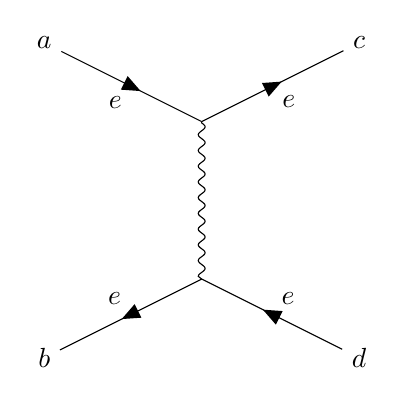
\begin{tikzpicture}
  \begin{feynman}
    \vertex (a) at (0,0) {$a$};    
    \vertex [below=4cm of a](b){$b$};
    \vertex [below right=1cm and 2cm of a](x);
    \vertex [below=2cm of x](y);
    \vertex [right=4cm of a](c){$c$};
    \vertex [below=4cm of c](d){$d$};    
    \diagram*{
      (a) -- [fermion, edge label'={$e$}] (x) -- [fermion,  edge label'={$e$}] (c),
      (d) -- [fermion, edge label'={$e$}] (y) -- [fermion,  edge label'={$e$}] (b),
      (x) -- [boson] (y)      
    };
\end{feynman}
\end{tikzpicture} &
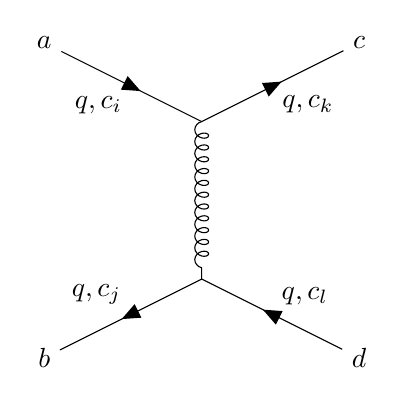
\begin{tikzpicture}
  \begin{feynman}
    \vertex (a) at (0,0) {$a$};    
    \vertex [below=4cm of a](b){$b$};
    \vertex [below right=1cm and 2cm of a](x);
    \vertex [below=2cm of x](y);
    \vertex [right=4cm of a](c){$c$};
    \vertex [below=4cm of c](d){$d$};    
    \diagram*{
      (a) -- [fermion, edge label'={$q, c_i$}] (x) -- [fermion,  edge label'={$q, c_k$}] (c),
      (d) -- [fermion, edge label'={$q, c_l$}] (y) -- [fermion,  edge label'={$q, c_j$}] (b),
      (x) -- [gluon] (y)      
    };
\end{feynman}
\end{tikzpicture}\\
QED & QCD \\
\end{tabular}
\end{center}
The corresponding matrix elements are:
$$\mathcal{M}_{\rm QED} = -\frac{e^2}{t}\big(\bar u(c)\gamma^\mu u(a)\big)\big(\bar v(b)\gamma_\mu v(d)\big)$$
and
$$\mathcal{M}_{\rm QCD} = -\frac{g_s^2}{t}\, T^a_{ki}\, T^a_{jl}\, \big(\bar u(c)\gamma^\mu u(a)\big)\big(\bar v(b)\gamma_\mu v(d)\big)$$
In the low energy limit, the QED process reduces to the familiar Coloumb potential:
$$V_{\rm QED} = - \frac{e^2}{4\pi r}$$
By comparing the two Matrix elements we expect that the corresponding low-energy limit for QCD is:
$$V_{\rm QCD} = - \frac{g_s^2}{4\pi r} T_{ki}^a T_{jl}^a$$
In the homework, you will show that the QCD potential is attractive for the color singlet state of the $q \bar{q}$ system and repulsive for a colored state. \\[5pt]

%\exercise (*) Show that the average of the color factor:
%$$T_{ki}^a T_{jl}^a$$
%is positive for the singlet color state:
%$$\tfrac{1}{\sqrt{3}}\Big( r\bar r + g\bar g + b\bar b \Big)$$
%and repulsive for the colored states:
%$$\tfrac{1}{\sqrt{2}}\Big( r\bar r - g \bar g \Big)$$
%and 
%$$\tfrac{1}{\sqrt{6}}\Big( r\bar r + g \bar g - 2 b \bar b\Big)$$
%you may use the Fierz Identity:
%\begin{equation}
%  \label{eqn:fierz}
%  \sum_a T^a_{ki}\, T^a_{jl} \;=\; \tfrac{1}{2}\delta_{il}\delta_{jk}
%                              \;-\; \tfrac{1}{6}\delta_{ki}\delta_{jl}.
%\end{equation}

\exercise (*) Show that fully antisymmetric 3-color state:
$$\tfrac{1}{\sqrt{6}}
\Big(rgb - rbg + gbr - grb + brg - bgr \Big)$$
is a color singlet, by applying the color raising operator $T_+$ with
$$T_+ r = g,  \quad T_+ g = 0, \quad T_+ b = 0.$$ 
and the color lowering operator:
$$T_- r = 0,  \quad T_- g = r, \quad T_- b = 0.$$ 
In principle, there are four more operators, but they have a similar results due to symmetry.




\end{document}
